
\section{Methodology}
\label{sec:methodology}
We begin with brief overview of elements used in this work to generate structural embeddings. 
This is followed by a detailed overview of the model used to jointly score documents and train 
structure embeddings. We compare the performance of the proposed architecture with some 
state-of-the-art learning to rank models. Finally, we provide a short description of the 
datasets and evaluation metrics used in this work.
\subsection{Structural Elements}
Web pages comprise of several structural elements. However, in this work we primarily study 
role of a small subset of structural elements in a webpage. We consider seven elements 
listed below.
\begin{enumerate}
\item \textbf{Headings:} Human beings use document or section headings as anchors 
or entry points \cite{} to paragraphs. Often headings summarize information conveyed by 
the text in the forthcoming paragraph, and can be treated as a separate element. 
\item \textbf{Tables:} The presence and contents of any tabular data in the 
document (table layout) is categorized in the Tables element. Certain type of 
information e.g. statistics, are easy to find in a table than scanning an  
entire document. In this work, we consider entire content in a table for learning 
its low-dimensional representation.
\item \textbf{Bold and Italics:} Any italicized or bold text is treated as a separate element. Often 
certain phrases are marked in bold text to convey their importance. 
All bold textual content is treated as a separate element.
\item \textbf{Hyperlinks:} Any reference to data (within the same document or 
across different web documents) that the reader can directly follow either by 
clicking, tapping, or hovering is considered as a hyperlink. We consider the 
anchor text of all hyperlinks present in a document under this element.
\item \textbf{Lists:} Authors often create ordered or unordered lists of content to summarize key points 
which in turn makes it easier for readers to parse information quickly. All textual 
content present in such lists is considered under the Lists structural element.
\item \textbf{Images:} Information items that are of a non-textual form, i.e., 
pictures or GIFs or videos comprise the Images entity category. In this work, we use meta-data 
contained in the image element to create embeddings. 
\end{enumerate}

It is important to analyze how these elements are distributed in a web corpus 
to approximate the quality of embeddings. Sparsely distributed elements that contain 
less textual content may not yield useful representations. Thus, we 
first analyze the distribution of above listed elements in Clueweb corpus labeled in 
TREC Web track 2011-2014. 
Figure \ref{fig:elements} presents the distribution of each of the seven 
structural elements listed above. We observe that hyperlinks and images are most 
common with over 90\% web documents containing at least one hyperlink or image. 
Specialized formats such as tables and lists are found in over 70\% of web 
documents.

In terms of formatting of textual content, bold texts and headings 
are much more commonly found in documents than italicized text, with less than 
30\% documents containing italicized text. In addition to the popularity of each 
element (Figure \ref{fig:elements}), we also look at the element co-occurrence 
patterns using a heatmap of co-occurring elements in Figure 
\ref{fig:heatmap}. We observe that Images are accompanied more by Hyperlinks in 
web documents than by Tables. Overall our analysis indicates myriad usage of 
structural elements in web documents in clueweb corpus. This re-emphasizes that 
these elements, if exploited, may indeed be useful in retrieval.  
% \textcolor{red}{TODO: did we normalize the values 
% per element? everything seems to go well with Hyperlinks! :P}
% \textcolor{green}{Per element? Its just $\frac{\sum 1(ele1)  \cap  
% 1(ele2)}{total_d}$ where $1(x)$ indicates whether x is present in d.}
    \begin{figure*}
    \centering
    \caption{Network architecture}
    \label{fig:network_architecture}
    \begin{subfigure}[b]{0.70\textwidth}
    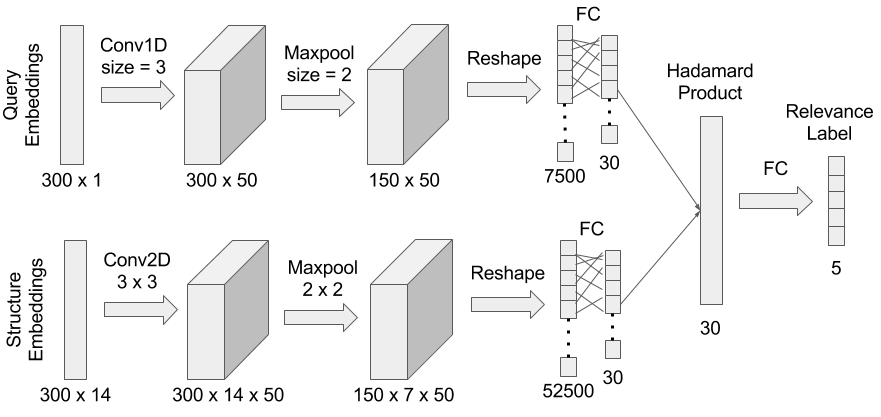
\includegraphics[width=\textwidth]{diagrams.png}
    \end{subfigure}
    \end{figure*}
\subsection{Retrieval with structure embeddings}
For preliminary analysis we rely on a simple convolutional neural 
network architecture that predicts both relevance of a document with 
respect to a search query and its structural embedding. 
The network architecture with each layer, input and output size 
is given in Figure \ref{fig:network_architecture}. 
Given $\mathit{Q}$ queries, $\mathit{D}$ documents in corpus and $\mathit{S}$ 
structural elements in a webpage, the model projects a query 
and document into an embedding space before scoring.

The proposed network has two input vectors: query and document. We represent each 
query $q_i \in \mathit{Q}$ query with 300\footnote{300 dimensional 
embeddings are standard in practice 
\cite{mitra2015query,zamani2016estimating}} dimensional vector. 
In this experiment, we represent each document $d_j \in \mathit{D}$  
with a stacked two-dimensional matrix, where each row is the embedding 
of $s_k \in \mathit{S}$ structural element. 
\begin{table}
  \centering
 \caption{Query and label distribution of 2011-2014 Web track}
 \label{table:data_distribution} 
 \begin{tabular}{|c|c|c|c|}
\hline
Year	&	\#q	&	\#docs	&	\#rel	 \\ \hline
2011	&	50	&	19381	&	3157		\\ \hline
2012	&	50	&	16102	&	3523		\\ \hline
2013	&	50	&	14531	&	4149		\\ \hline
2014	&	50	&	14610	&	5665		\\ \hline
 \end{tabular}
\end{table}

Each query vector is first passed through one-dimensional convolutional
layer with 50 filters, kernel size of 3 and stride of 1. 
However, each document vector is first passed through a two-dimensional convolutional
layer with 50 filters, a kernel size of 3X3, and a stride of 1. 

While, output of query convolution layer is further passed into a size 2 pooling 
layer, output of document convolution layer is passed into size 2x2 pooling layer.  
This is followed by reshaping and a final fully-connected layer 
that produces a single real-valued vector. 
All the nodes in the model use the rectified linear unit (relu) function 
for non-linearity.

\begin{table*}
 \caption {$NDCG@$1 and $NDCG@$10 for 2011-2014 }
 \label{table:network_perf} 
 \begin{tabular}{|c||c|c|c|c||c|c|c|c|} \hline
& \multicolumn{4}{|c|}{NDCG@1} &  \multicolumn{4}{|c|}{NDCG@10} \\ \hline
System &  2011 & 2012  & 2013 & 2014 &  2011 & 2012  & 2013 & 2014 \\ \hline
$SVM_r$ & \textbf{0.25} & \textbf{0.16} & 0.23 & 0.17 & \textbf{0.26} & 0.13 & 0.27 & 0.23   \\
$LMart$ & 0.23 & 0.10 & 0.22 & \textbf{0.27} & 0.24 & \textbf{0.16} & 0.30 & \textbf{0.29} \\
$SEmbed_{all}$   & 0.21$^\downdownarrows$ & 0.11$^\downdownarrows$ & \textbf{0.24$^*$}  & 0.25$^\upuparrows$ & \textbf{0.26} & 0.15$^*$ & \textbf{0.32}$^\upuparrows$ & \textbf{0.29}$^\upuparrows$\\ \hline 
$SEmbed_{head}$  & 0.05 & \textbf{0.10}$^\downdownarrows$ & \textbf{0.16}$^\downdownarrows$ & 0.13$^\downdownarrows$ & 0.08$^\downdownarrows$ & \textbf{0.14}$^\downdownarrows$ & \textbf{0.17}$^\downdownarrows$ & 0.16$^\downdownarrows$ \\ 
$SEmbed_{table}$ & \textbf{0.08}& 0.05$^\downdownarrows$& 0.09$^\downdownarrows$ & 0.13$^\downdownarrows$ & 0.07$^\downdownarrows$ & 0.09$^\downdownarrows$ & 0.14$^\downdownarrows$ & 0.19$^\downdownarrows$ \\
$SEmbed_{link}$  & 0.06& 0.05$^\downdownarrows$& 0.12$^\downdownarrows$& \textbf{0.24}$^\upuparrows$ & \textbf{0.10}$^\downdownarrows$ & 0.10$^\downdownarrows$ & 0.15$^\downdownarrows$ & \textbf{0.21}$^\downdownarrows$  \\ 
$SEmbed_{list}$  & 0.05& 0.05$^\downdownarrows$& 0.10$^\downdownarrows$ & 0.14$^\downdownarrows$ & 0.09$^\downdownarrows$ & 0.11$^\downdownarrows$ & 0.15$^\downdownarrows$ & 0.17$^\downdownarrows$\\ 
$SEmbed_{img}$   & 0.03& 0.05$^\downdownarrows$& 0.13$^\downdownarrows$& 0.15$^\downdownarrows$ & 0.08$^\downdownarrows$ & 0.10$^\downdownarrows$ & 0.16$^\downdownarrows$ & 0.20$^\downdownarrows$ \\ \hline
\end{tabular}
\\
\footnotemark{p-val: $^*$ $\le$ 0.05,  $^\upuparrows$ $\le$ 0.001, $^\downdownarrows$ $\le$ 0.001 over SVMRank with paired t-test}
 \end{table*}
We compute the posterior probability of document relevance given a query 
from the semantic relevance score between them
through a softmax function in Equation \ref{eq:activation}. 
\begin{equation}
\label{eq:activation}
  p(R_{d_j} = r|q_i) = \frac{e^{\beta_r * f(q_i, d_j)}} {\sum_{0<c<K}e^{\beta_c * f(q_i, d_j)}}
\end{equation}

where $P(R_{d_j}=r|q_i)$ is the probability that relevance grade $R_{d_j}$ of 
document $d_j$ for query $q_i$ is $r$. $K$ represents different 
relevance grades in training data.

Given $M$ query, document pair and corresponding relevance label as 
training data, we optimize the cross-entropy loss 
function in Equation \ref{eq:loss_func}. 
\begin{equation}
 \label{eq:loss_func}
 \mathcal{L}(x;\theta) = - \frac{1}{n} \sum_{0<n<M}\sum_{0<c<K} 
    [ r_j ln ( \hat r_j) + (1 -  r_j)ln(1 - \hat r_j)]
\end{equation}
where $r_j$ and $\hat r_j$ are actual and predicted relevance labels of a document 
for a query respectively. $K$ represents different relevance grades in training data. 

We generate initial query and document embeddings using 
glove\footnote{https://nlp.stanford.edu/projects/glove/}. We generate embedding for each 
query by computing the average of its term embeddings. We create two dimensional 
document embeddings by stacking average term embeddings of the seven structural elements
listed above. 

The output of fully connected layer just after reshaping layer in Figure \ref{fig:network_architecture} 
would represent low dimensional structure embeddings for each document. 
Thus, in future, we shall investigate the utility of these embeddings for 
tasks other than retrieval. 

\subsection{Dataset}
We rely on TREC Web collection (2011-2014) \cite{collins2015trec} for 
our experiments. Table \ref{table:data_distribution} shows the distribution of 
relevance labels per year. 

We use 3 TREC Web datasets (150 queries)\footnote{Further divided into 4:1 
ratio for training and validation sets} to train and one dataset (50 queries) to test 
its effectiveness. For example, results for 2014 TREC web queries are obtained 
by training on 2011-2013 TREC web queries as training data. 

\subsection{Baselines}
Several algorithms exist
in the literature that optimize for relevance. In recent years, learning-to-rank 
approaches such as RankSVM \cite{Cao2006Sigir} and LambdaMart 
\cite{Burges2010Report} have proved to be effective in optimizing metrics such 
as NDCG. Thus, in this work we  compare the proposed model with both SVMRank and 
LambdaMart. 

LambdaMart \cite{Burges2010Report}  (\textbf{LMart}) relies on boosted 
regression trees to optimize non-smooth IR metrics such as NDCG. It has been 
extensively used in ranking tasks and also won Yahoo! Learning to rank 
challenge \cite{Chapelle2011Yahoo} in 2010. 
SVMRank \cite{Cao2006Sigir} ({$\boldsymbol{SVM_r}$}), a pairwise max-margin 
approach is used to learn a function to rank documents for a query. Given a set 
of document labels, query and document feature vectors, 
SVMRank optimizes the objective function learns a hyperplane that 
enforces ordering among relevant and non-relevant documents. 

Above approaches require hand-crafted features. We rely on features used in 
Letor \cite{liu2007letor}, a popular dataset which consists of several query, document text 
and structure specific features. For this preliminary work, we computed 68 
features to train and test these models.

\subsection{Evaluation metric}
\label{sec:evaluation}
There are several metrics that can be used to evaluate effectiveness of an IR 
system. 
In this work we rely on Normalized Discounted Cumulative Gain (NDCG) 
\cite{Jarvelin2000NDCG} 
to evaluate different systems. NDCG score at position $n$ is calculated as 
follows: 
\begin{equation}
 NDCG@n = Z_n \sum_{j=1}{n} \frac{2^{y_j} - 1}{log_2 j + 1}
\end{equation}
where $j$ is the position in the document list, $y_j$ is the label (relevance or 
effort) of 
the document $d_j$ in the list and $Z_n$ is the normalization factor which is 
the oracle 
discounted cumulative gain at position $n$ so that a perfect list gets NDCG 
score of 1.
